% Chapter Template

\chapter{ESTUDIO DE LAS PROPIEDADES MECANICAS DE UN BMG POROSO SINTERIZADO (NANOVIDRIOS)} % Main chapter title

\label{C5} % Change X to a consecutive number; for referencing this chapter elsewhere, use \ref{ChapterX}

\lhead{Capítulo 5. \emph{ESTUDIO DE LAS PROPIEDADES MECANICAS DE UN BMG POROSO SINTERIZADO (NANOVIDRIOS)}} % Change X to a consecutive number; this is for the header on each page - perhaps a shortened title


%----------------------------------------------------------------------------------------
%	SECTION 1
%----------------------------------------------------------------------------------------

\section{Introducción}
\label{S5_1}

% Un vidrio metálico (MG), también llamado ``metal amorfo'', es una aleación metálica que posee una estructura amorfa,
% en oposición a la estructura cristalina que normalmente presentan los metales. Esto puede lograrse mediante varias técnicas,
% la mayoría de las cuales incluyen altas velocidades de temple, peque\~nos volúmenes y el control de la composición del
% material \citep{liebermann93}. Como resultado, estos materiales cuentan con algunas ventajas con respecto a los metales cristalinos:
% mejor elasticidad combinada con una alta resistencia, dureza y moldeabilidad \citep{telford04}.

% Existen dos enfoques principales para simular vidrios metálicos sometidos a deformación plástica: haciendo foco en el comportamiento
% a escala nanométrica \citep{ogata06,guan10} o utilizando mecánica del continuo \citep{malvern69}. Para el primer enfoque, las simulaciones
% con dinámica molecular (MD) son frecuentemente utilizadas \citep{allen87}. La dinámica molecular puede resolver problemas en los cuales
% interactuan muchos cuerpos (átomos), mediante la aplicación de un potencial entre pares de átomos. Así, este enfoque es útil para el
% estudio de propiedades a escala nanométrica, tal como la deformación, la tensión, la temperatura, etc.

% Las simulaciones con dinámica molecular también son útiles para identificar procesos pláticos en BMGs. La plasticidad comienza con la
% formación de zonas de transformación de tensión cortante (STZ), las cuales se nuclean, formando bandas de corte \citep{ogata06,shimizu07} a medida que la
% deformación aumenta. Las bandas de corte (SB) pueden provocar la falla frágil del material debido a la deformación heterogénea. De allí la importancia
% de prevenir o retrasar su propagación. En los metales cristalinos se procede de forma similar al trabar las dislocaciones.

Los vidrios metálicos con porosidad han sido objeto de mucho estudio en los últimos años \citep{guan13,wang10}, en un esfuerzo
por mejorar el entendimiento de su mecánica de deformación. El comportamiento en el
régimen elastoplástico puede ser controlado mediante la introducción de poros.

Las grandes deformaciones normalmente se deben, como se ha visto en capítulos anteriores, al colapso de zonas de transformación de
tensión cortante (STZ) que dan lugar a una o varias bandas de corte (SB), las cuales pueden provocar la falla frágil del material debido a la
deformación heterogénea. De allí la importancia de prevenir o retrasar su propagación.

La adición de poros en metales cristalinos reduce, como es sabido, el movimiento de dislocaciones y modifica la
deformación plástica resultante. De igual manera, los poros en vidrios metálicos limitan la propagación de bandas de corte y permiten
una deformación más homogénea. Ultimamente, se ha suscitado un gran interés al respecto, y varias opciones han sido exploradas
\citep{guan13,wang10,schuh07,liontas14}.

En el presente capítulo fabricamos muestras de BMG Cu$_{46}$ Zr$_{54}$ con porosidad
(similar a las muestras de ``nanovidrios'' en otros experimentos y simulaciones \citep{adibi13,albe13}) mediante el sinterizado de nanopartículas.
Las simulaciones con dinámica molecular nos permitirán analizar los polyedros de Voronoi, las tensiones y deformaciones atómicas,
así como también la forma en que la porosidad inicial afecta la deformación resultante de la muestra.

% En un trabajo previo hemos determinado los parámetros constitutivos del vidrio metálico Cu$_{46}$ Zr$_{54}$ como
% una función de la temperatura. Ahora presentamos resultados para un vidrio metálico de igual composición, pero
% fabricado mediante el sinterizado de nanopartículas de BMG, lo cual resulta en muestras con porosidad, similar
% a las muestras de ``nanovidrios'' en otros experimentos y simulaciones \citep{adibi13,albe13}. Para llevar a cabo las simulaciones atomísticas
% hemos utilizado el enfoque de Dinámica Molecular (MD), y el estudio incluye análisis de los polyedros de Voronoi, tensiones
% y deformaciones atómicas. Analizamos de qué forma depende la deformación en la fracción de volumen sólido (SVF), y cómo la deformación
% se distribuye a lo largo de la muestra en función de la porosidad inicial.

% Una deformación más homogénea puede ser lograda mediante el agregado de nanoinclusiones al material. Ultimamente, se ha suscitado
% un gran interés al respecto, y varias opciones han sido exploradas \citep{guan13,wang10,schuh07,liontas14}. Siguiendo trabajo previo, en el
% presente trabajo fabricamos muestras de BMG Cu$_{46}$ Zr$_{54}$ con porosidad (similar a las muestras de ``nanovidrios'' en otros
% experimentos y simulaciones \citep{adibi13,albe13}) mediante el sinterizado de nanopartículas. Las simulaciones con dinámica molecular
% nos permitirán analizar los polyedros de Voronoi, las tensiones y deformaciones atómicas, así como también la forma en que la porosidad inicial
% afecta la deformación resultante de la muestra.

%----------------------------------------------------------------------------------------
%	SECTION 2
%----------------------------------------------------------------------------------------

\section{Detalles de Simulación y Preparación de la Muestra Porosa}
\label{S5_2}

% Para este trabajo, las simulaciones con dinámica molecular fueron realizadas mediante el uso del programa LAMMPS \citep{plimpton95},
% el cual es gratuito y de código libre, tiene un muy buen manual y es computacionalmente eficiente para la simulación de sistemas
% con gran número de átomos. Por otro lado, el análisis de Voronoi y las imágenes de la muestra fueron realizadas con el programa Ovito
% \citep{stukowski10}, y otras figuras fueron graficadas con Gnuplot. Ambos programas son gratuitos y de código libre.

\begin{figure}[h!]
  \centering
  \begin{tabular} {c}
    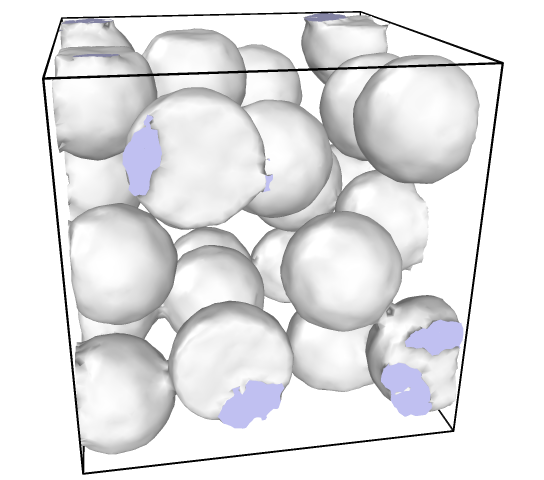
\includegraphics[width=10cm]{Cap_5/spheres2.png}\\
    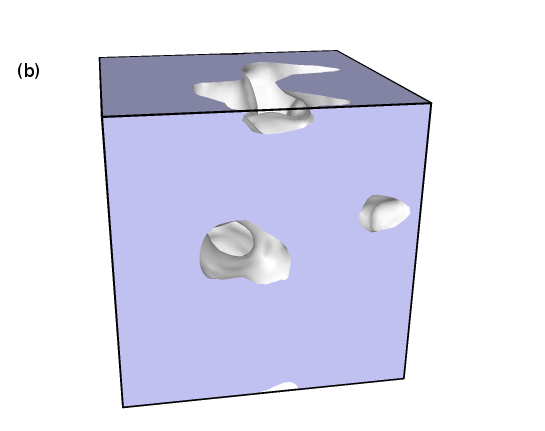
\includegraphics[width=10cm]{Cap_5/spheres3.png}\\
  \end{tabular}
  \caption[Imágenes de la muestra]{Imágenes de la muestra (a) anterior al proceso de sinterizado y (b) posterior
  al proceso de sinterizado (porosidad 13\%).}
  \label{C5:fg:sint}
\end{figure}

Para la preparación de la muestra porosa, hemos tomado como punto de partida la misma muestra utilizada con anterioridad (capítulo \ref{C3}).
% y descripta por \cite{arman10}. Se trata de una muestra prismática Cu$_{46}$ Zr$_{54}$ con un total de 160000 átomos y obtenida
% mediante una velocidad de enfriamiento de 10$^{12}$ K/s. La temperatura de transición vítrea experimental (T$_{g}$) de este vidrio metálico
% es de 696 K, y el módulo de cizalladura (o módulo de elasticidad transversal G) es 30 GPa \citep{johnson05}. 
Para describir las interacciones
entre los átomos, usamos nuevamente el potencial EAM (método de átomo embebido) \citep{daw84}. Usamos condiciones de frontera periódicas en las
tres caras, lo cual es apropiado para altas velocidades de deformación \citep{bringa05}. De esta forma, podemos simular un BMG (de mayor tamaño)
y evitar concentración de tensiones en las fronteras.

Tomamos la muestra original y la replicamos a modo de obtener una muestra aproximadamente cúbica, de 15 nm de lado. Luego, seleccionamos puntos
al azar dentro de la muestra para hacer de centro de las esferas (de 2.5 nm de radio), y removimos todo el material al exterior de dichas esferas
para simular el sinterizado de nanopartículas esféricas de material. La figura~\ref{C5:fg:sint}-(a) muestra el resultado de estas acciones. Esta
nueva muestra tiene 77888 átomos.

El procedimiento para simular el sinterizado fue de relajar la muestra a una temperatura constante de 650K, justo debajo de la temperatura
de transición vítrea, y volúmen constante durante unos pocos ps, y luego aplicar hasta 10 ps de presión compresiva (400 bar). Estos dos pasos
fueron repetidos hasta lograr las porosidades deseadas. Luego, relajamos la muestra una vez más mediante el siguiente procedimiento: temple a 
temperatura cero mediante una velocidad de enfriamiento de $6.5 \cdot 10^{14} K/s$, aplicación de un baróstato para llegar a presión
cero, calentamiento a la misma velocidad que la velocidad de enfriamiento para llegar a la temperatura de simulacion (300K) y,
finalmente, aplicación de un baróstato durante 5 ps para reducir la presión a cero mientras se mantiene la temperatura constante. La 
figura~\ref{C5:fg:sint}-(b) exhibe una de las muestras obtenidas mediante el proceso que se ha explicado.

Se prepararon muestras con distintas porosidades iniciales (3.3\%, 5.8\% y 13.1\%). Estas muestras estabilizadas fueron luego utilizadas
para realizar carga uniaxial de compresión y tracción. Todas las coordenadas atómicas fueron recalculadas cada paso, en relación con la
velocidad de deformación requerida, la cual fue de $10^9 /s$, valor apropiado para experimentos de choque compresivo.

%----------------------------------------------------------------------------------------
%	SECTION 3
%----------------------------------------------------------------------------------------

\section{Resultados}
\label{S5_3}

A continuación presentamos resultados para deformación puramente uniaxial, la cual es adecuada para realizar comparaciones con resultados de
experimentos a altas velocidades de deformación, donde las deformaciones laterales pueden ser despreciadas.

\begin{figure}[h!]
  \centering
  \begin{tabular} {c}
    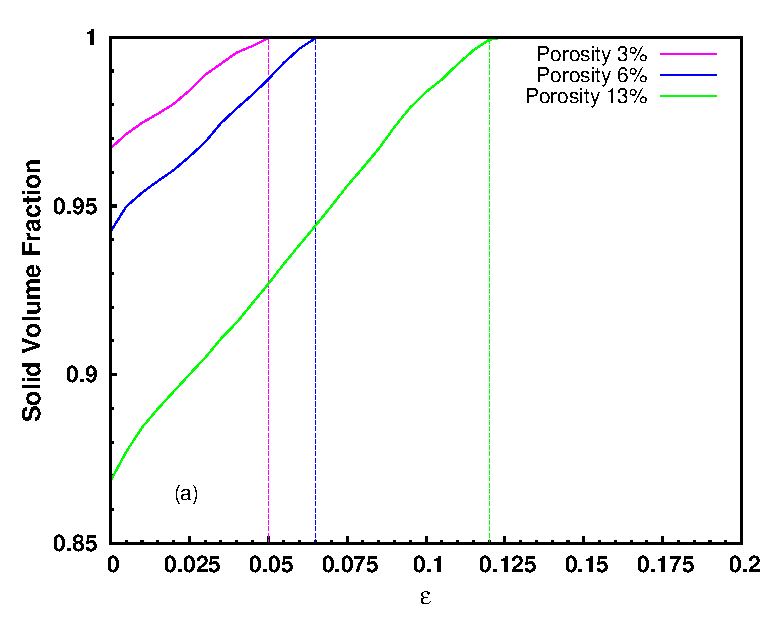
\includegraphics[width=10cm]{Cap_5/SVF_strain_comp_dash.eps}\\
    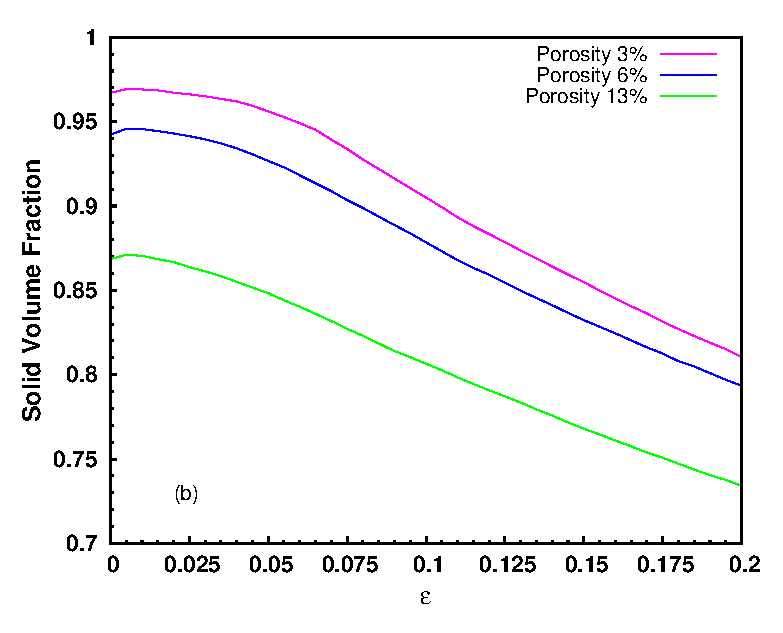
\includegraphics[width=10cm]{Cap_5/SVF_strain_tens.eps}\\
  \end{tabular}
  \caption[Fracción de volumen sólido (SVF) versus deformación.]{Fracción de volumen sólido (SVF) versus deformación. (a) Compresión
  (b) Tracción. En (a), las líneas a trazos indican la deformaión a la cual los poros se cierran por completo}
  \label{C5:fg:svf}
\end{figure}

La figura~\ref{C5:fg:svf} muestra la evolución de la densidad en las muestras porosas. Para el caso de compresión, hemos agregado unas líneas a trazos
que indican el punto en el que los poros se cierran completamente, es decir, la fracción de volumen sólido es igual a 1.
Para cada porosidad, el valor de deformación $\epsilon$ correspondiente es: 3\% $\rightarrow$ 0.05, 6\% $\rightarrow$ 0.065, 13\% $\rightarrow$ 0.12.
En algunas de las figuras de esta sección aparecerán estas líneas nuevamente, a fin de observar si este evento implica cambios en el comportamiento
plástico. Para el caso de tracción, el uso de condiciones de borde periódicas evita que los poros se cierren incluso a altas
deformaciones uniaxiales, dado que no hay deformaciones laterales.

\begin{figure}[h!]
  \centering
  \begin{tabular} {c}
    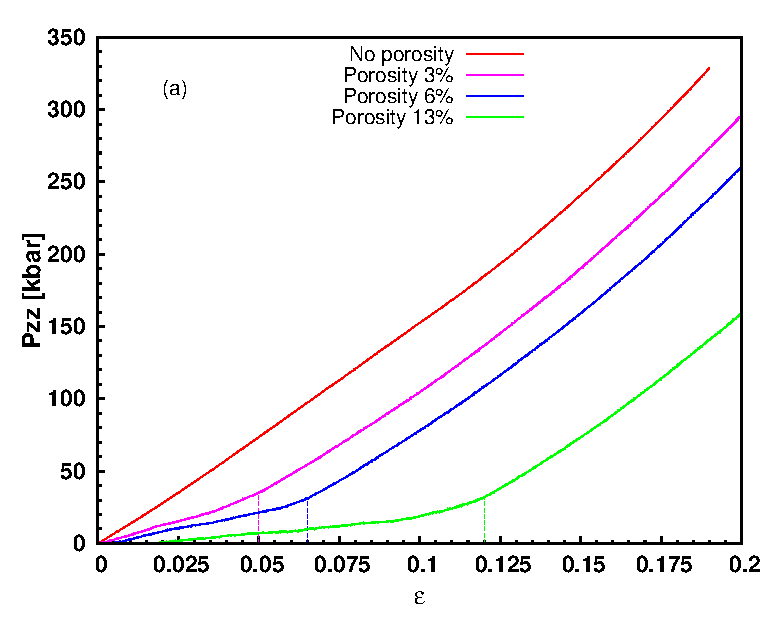
\includegraphics[width=10cm]{Cap_5/Pzz_strain_comp_dash.eps}\\
    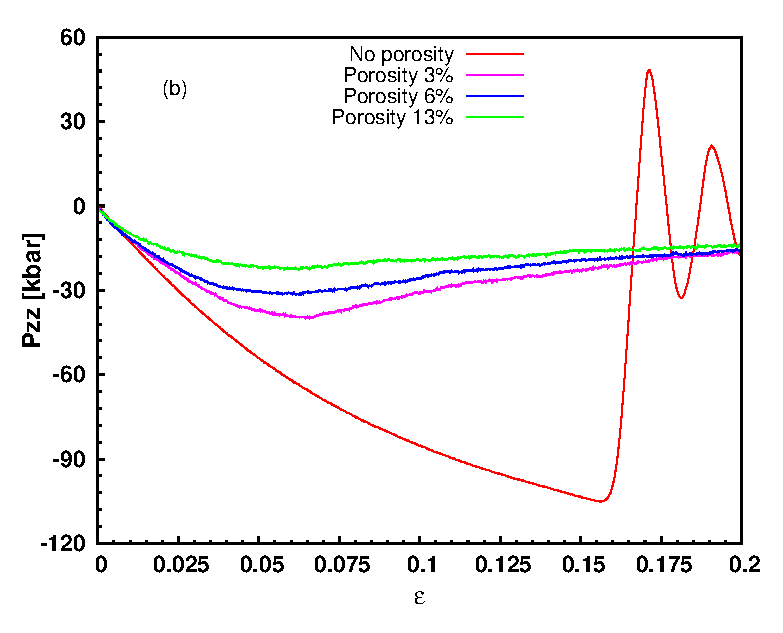
\includegraphics[width=10cm]{Cap_5/Pzz_strain_tens.eps}\\
  \end{tabular}
  \caption[Presión en el eje Z vs deformación.]{Presión en el eje Z vs deformación. (a) Compresión (b) Tracción.}
  \label{C5:fg:pzz2}
\end{figure}

\begin{figure}[h!]
  \centering
  \begin{tabular} {c}
    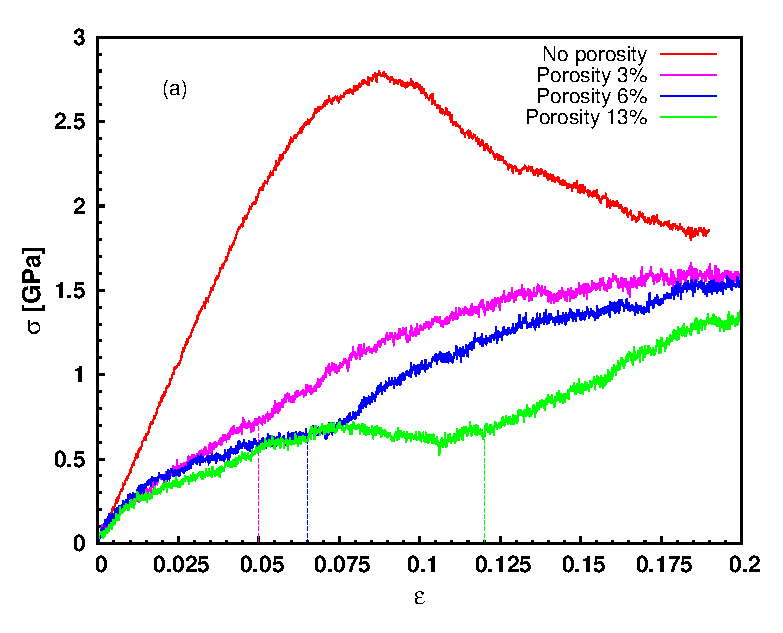
\includegraphics[width=10cm]{Cap_5/stress_strain_comp_dash.eps}\\
    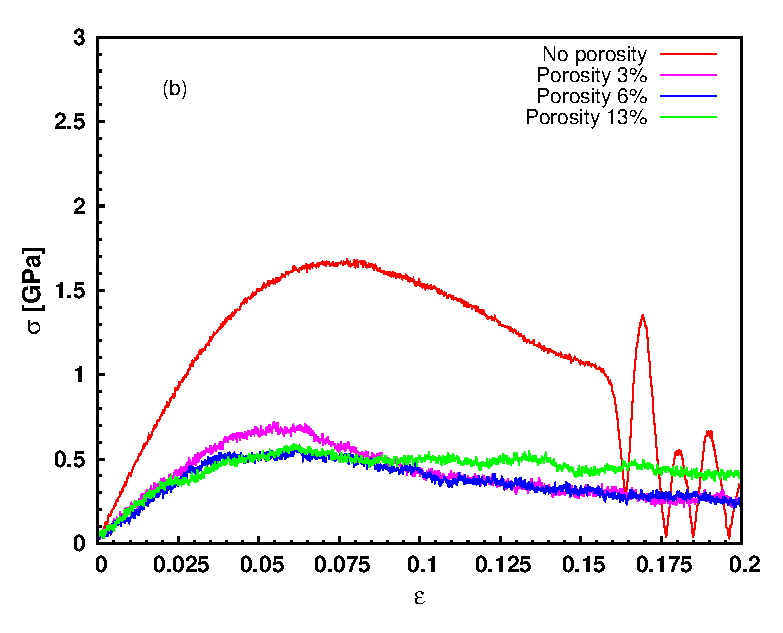
\includegraphics[width=10cm]{Cap_5/stress_strain_tens.eps}\\
  \end{tabular}
  \caption[Tensión de von Mieses vs deformación.]{Tensión de von Mieses vs deformación. (a) Compresión (b) Tracción.}
  \label{C5:fg:stress}
\end{figure}

La figura~\ref{C5:fg:pzz2}-(a) grafica la presión en el eje de carga versus deformación para esfuerzos de compresión. La figura~\ref{C5:fg:stress}-(a),
a su vez, grafica el esfuerzo de von Mieses versus deformación para esfuerzos de compresión.
Ambas gráficas nos indican que la presencia de porosidad promueve el inicio de la plasticidad. Los poros actúan como concentradores de tensión,
facilitando la aparición de STZs y bandas de corte. Esta plasticidad temprana comienza a
cerrar los poros, produciendo una curva donde la deformación $\epsilon$ aumenta mientras que la presión se mantiene baja.
Cuando los poros se cierran, la presión aumenta más aceleradamente, como puede apreciarse en la porción de la curva posterior
a la línea de trazos. Podemos también observar que el comportamiento de las muestras porosas luego de las líneas de trazos es
muy similar al comportamiento de la muestra sin porosidad, validando el hecho de que a ese punto ya no hay más porosidad. Basándonos en la figura,
podemos concluir que a mayor porosidad, se necesita menor esfuerzo para cerrar los poros (denotado por la altura de las líneas a trazos),
pero esto ocurre a mayores deformaciones.

En tracción las muestras se comportan diferentemente. Como ya se ha dicho los poros no se cierran en tracción, como sí lo hacían en compresión.
Mediante el análisis de algunas imágenes de la muestra, como las que aparecen en la figura~\ref{C5:fg:ss_tens},
observamos que los poros crecen a una velocidad aproximadamente constante a medida que la deformación de la muestra aumenta. 
Las figuras~\ref{C5:fg:pzz2}-(b) y \ref{C5:fg:stress}-(b) también muestran lo que parece ser flujo plástico: particularmente a 13\% porosidad,
pero similarmente a otras porosidades, luego de un cierto punto, la deformación aumenta mientras la presión se mantiene constante o
incluso disminuye.

\begin{figure}[h!]
  \centering
  \begin{tabular} {c}
    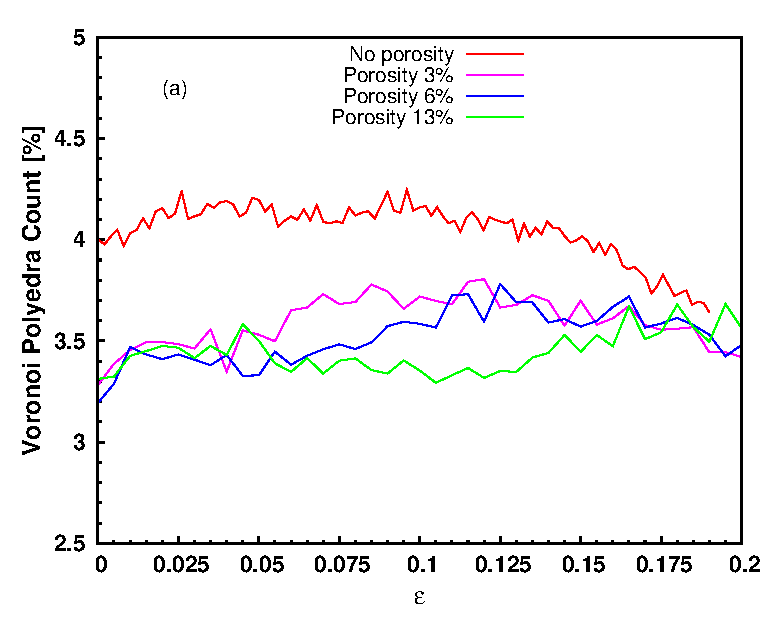
\includegraphics[width=10cm]{Cap_5/tipe3_strain_comp.eps}\\
    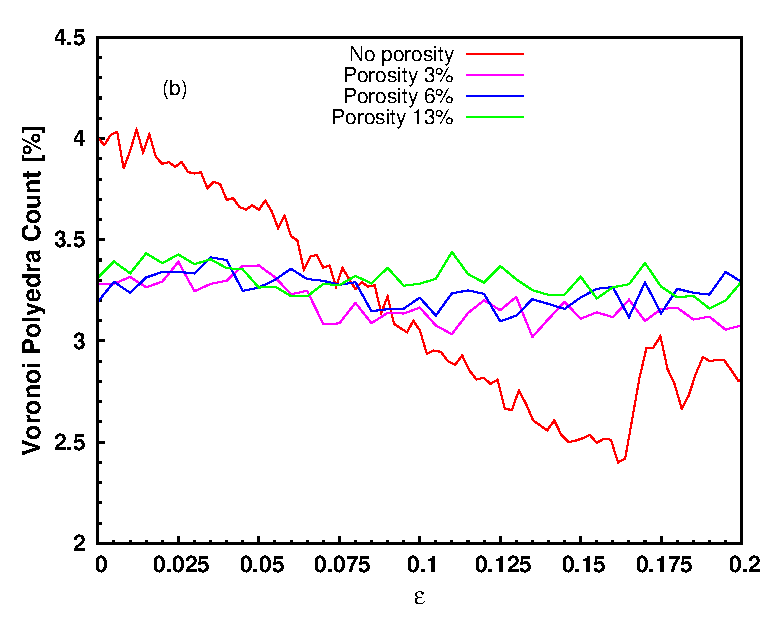
\includegraphics[width=10cm]{Cap_5/tipe3_strain_tens.eps}\\
  \end{tabular}
  \caption[Polyedros de Voronoi tipo 3 vs deformación.]{Polyedros de Voronoi tipo 3 vs deformación. (a) Compresión (b) Tracción.}
  \label{C5:fg:tip3}
\end{figure}

\begin{figure}[h!]
  \centering
  \begin{tabular}{c}
    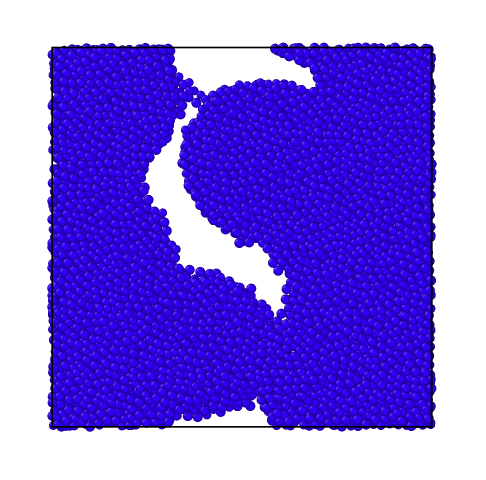
\includegraphics[width=8cm]{Cap_5/13_0strain.png} \\
    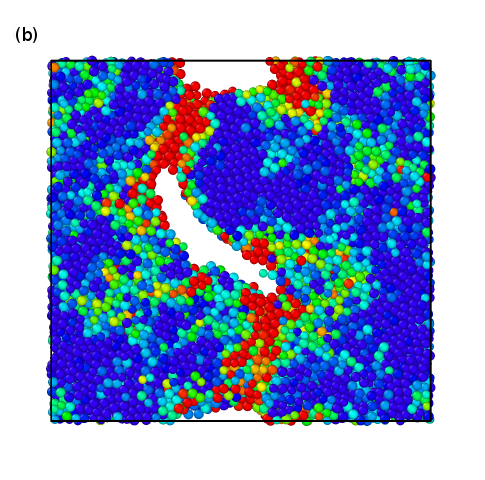
\includegraphics[width=8cm]{Cap_5/13_5strain_comp.png}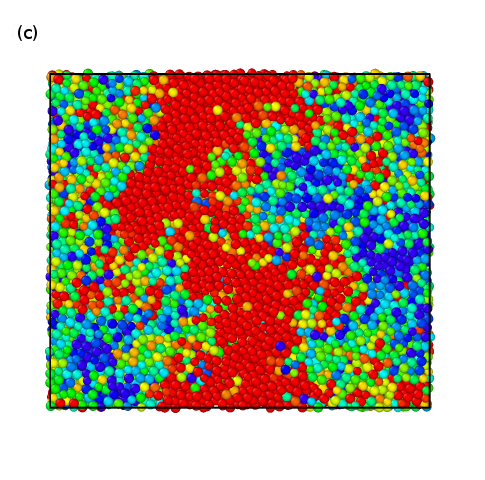
\includegraphics[width=8cm]{Cap_5/13_12strain_comp.png} \\
  \end{tabular}
  \caption[Coloreado de una sección de la muestra con porosidad 13\% según la deformación cortante.]{Coloreado de una sección de la muestra con
  porosidad 13\% según la deformación cortante. El coloreado fue hecho usando Ovito, el color azul siendo 0.1 o menor y el color rojo 0.3 o mayor.
  (a) Estado inicial de la muestra (b) 5\% deformación por compresión (c) 12\% deformación por compresión.}
  \label{C5:fg:ss_comp}
\end{figure}

\begin{figure}[h!]
  \centering
  \begin{tabular}{c}
    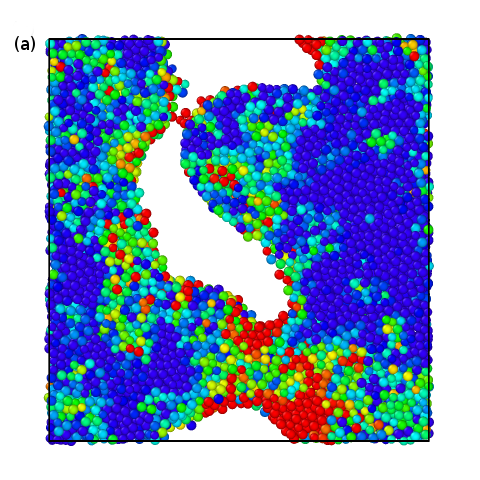
\includegraphics[width=8cm]{Cap_5/13_6strain_tens.png}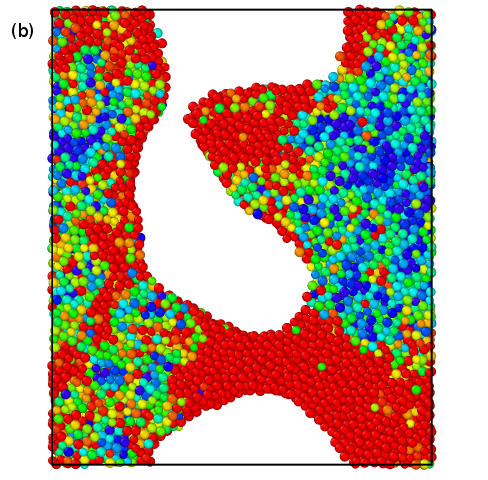
\includegraphics[width=8cm]{Cap_5/13_20strain_tens.png} \\
  \end{tabular}
  \caption[Coloreado de una sección de la muestra con porosidad 13\% según la deformación cortante.]{Coloreado de una sección de la muestra con
  porosidad 13\% según la deformación cortante. El coloreado fue hecho usando Ovito, el color azul siendo 0.1 o menor y el color rojo 0.3 o
  mayor. (a) 6\% deformación por tracción (b) 20\% deformación por tracción.}
  \label{C5:fg:ss_tens}
\end{figure}

La figura~\ref{C5:fg:tip3} muestra curvas de polyedros de Voronoi versus deformación. El análisis por teselado de Voronoi es una técnica para
caracterizar el ordenamiento local en vidrios metálicos amorfos, donde cada átomo es el centro de un polyedro de Voronoi,
completado por sus vecinos más cercanos. En \cite{arman10}, los átomos de tipo 3 son identificados como indicadores de plasticidad, por eso
son de gran importancia.

La figura~\ref{C5:fg:tip3}-(a) presenta las curvas de polyedros de Voronoi para esfuerzos de compresión. El gráfico muestra una caída en el número
de los átomos tipo 3, la cual sucede luego de una fase constante. Se ha pensado en este fenómeno como un indicador del inicio de la plasticidad
\citep{arman10}. Sin embargo, nuestras curvas muestran un resultado contraintuitivo, ya que la plasticidad comienza antes en las muestras con menor
porosidad de acuerdo a nuestro análisis. Esto podría ser considerado como un indicador de que hay otros factores o procesos en juego que afectan
los resultados.

Las figuras~\ref{C5:fg:ss_comp}-(b) y (c) presentan la evolución de la deformación cortante en la muestra, para esfuerzos de compresión.
Salta inmediatamente a la vista que los poros actúan como concentradores de tensiones, pero también representan un obstáculo para la
propagación de bandas de corte \citep{wang10}. Las bandas de corte nuclean diagonalmente en el espacio entre poros, y la deformación atómica
se acumula a lo largo de estas direcciones principales por el resto de la simulación, como puede observarse en la imágen de la muestra a 
deformación 12\%. Un endurecimiento de la muestra ocurre algunos momentos previo al cierre total de los poros, tal y como a apreciado
\cite{yuan14} y puede verse en la figura~\ref{C5:fg:pzz2}-(a).

La figura~\ref{C5:fg:tip3}-(b) muestra las curvas de poledros de Voronoi para esfuerzos de tracción. En esta imágen, los átomos de tipo 3
prácticamente no varían en las muestras con porosidad, lo que implicaría que no hay formación de STZs.
Para la muestra no porosa, el número de átomos tipo 3 se vuelve aproximadamente constante luego de que se ha nucleado el poro. Esto
nos llevó a pensar que, dada las condiciones de las muestras, se facilita el movimiento de los átomos alrededor de los poros, lo cual evita
la formación de STZs fuera de los alrededores de los poros. Para apoyar esta idea, en las figuras~\ref{C5:fg:ss_tens}-(b) y (c) presentamos
la muestra coloreada con la deformación cortante. Es evidente que la deformación cortante se concentra principalmente alrededor
de los poros. Debe ser mencionado que la posición relativa entre átomos que se encuentran lejanos de los poros se mantiene aproximadamente igual.


%----------------------------------------------------------------------------------------
%	SECTION 4
%----------------------------------------------------------------------------------------

\section{Conclusiones}
\label{S5_4}

Se realizaron simulaciones de Dinámica Molecular (MD) en una muestra porosa del vidrio metálico Cu$_{46}$ Zr$_{54}$, aplicando esfuerzos
de compresión y tracción. Los resultados bajo deformación fueron comparables a aquellos encontrados en la literatura \citep{yuan14} para
la compresión de muestras porosas de monocristales de cobre. Esto puede ser considerado como una validación del proceso de sinterizado 
utilizado para la preparación de las muestras.

Con carga compresiva, los poros facilitan la plasticidad actuando como concentradores de tensiones, pero también retrasan
la formación de zonas de transformación de tensión cortante (STZs) y su posible unión en una banda de corte (SB), para el material lejano a los poros.
Los resultados también exhiben un endurecimiento de la muestra al cerrarse los poros, similarmente a lo que ocurre en el caso no poroso.

Con carga de tracción y deformación puramente uniaxial, los poros no cierran y concentran flujo plástico alrededor de ellos, a su vez
que también impiden la formación de STZs y bandas de corte.

% Estudios futuros incluirán un análisis de Voronoi profundizado y la simulación de muestras más grandes con topologías de porosidad diferentes.

